\documentclass[a4paper]{article}

\usepackage{a4wide}
\usepackage{amssymb}
\usepackage{xcolor}
\usepackage{comment}
\usepackage{graphicx}
\usepackage[dutch]{babel}

\title{Elektronisch stemmen \\ \large De ethische discussie over elektronisch stemmen in de digitale samenleving.}
\author{
Mick van Gelderen \\ 4091566 \and 
Mick de Lange \\ 1534068 \and
Salim Salmi \\ 4089715
}


\newcommand{\TODO}[1]{{\color{red}\textbf{TODO: #1}}}

\usepackage{amsmath}
\begin{document}

\thispagestyle{plain}
\maketitle

\hfill \\ \\ \\ \\ \\ \\ \\ \\ \\ \\
\begin{figure}[htp]
\centering
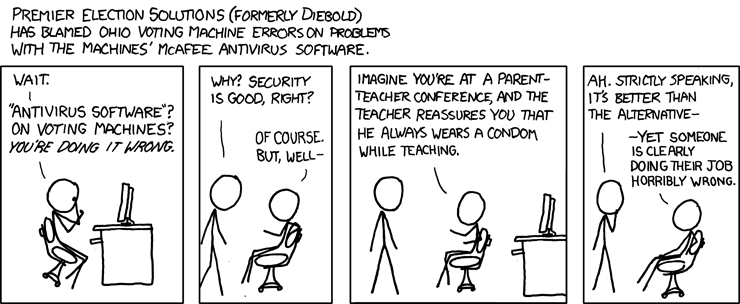
\includegraphics[width=\textwidth]{media/voting_machines.png}
\label{fig:voting-machines}
\begin{comment}
Randall Munroe, (2013), Voting Machines [ONLINE]. Available at: http://imgs.xkcd.com/comics/voting_machines.png [Accessed 15 March 13].
\end{comment}
\end{figure}

\newpage

\thispagestyle{plain}

\section*{Voorwoord}
Dit artikel is geschreven door 3 studenten Technische Informatica aan de Technische Universiteit Delft voor het vak `informatietechnologie en waarden'.
Het belicht een ethische kwestie van verschillende standpunten aangesterkt met literatuur uit het vakgebied en de filosofie. 

\section*{Samenvatting}

\newpage

\thispagestyle{plain}
\renewcommand{\contentsname}{Inhoud} 
\tableofcontents

\newpage

\section{Inleiding}

In de afgelopen jaren is er in Nederland veel te doen geweest rondom elektronisch stemmen.
Zo zijn er een aantal proeven geweest, met verschillende vormen van elektronisch stemmen.
Er zijn naar aanleiding van een aantal problemen actiegroepen opgericht die zich duidelijk uitspraken tegen elektronisch stemmen.
De overheid heeft uiteindelijk verschillende commissies ingesteld die onderzoek hebben gedaan naar de problemen en naar de benodigdheden om in de toekomst elektronisch stemmen in te voeren.

Er spelen binnen dit onderwerp verschillende technische en morele onderwerpen.
Veel genoemd zijn privacy en veiligheid, maar ook de mogelijkheid om bijvoorbeeld gemakkelijker en sneller de stemmen te tellen.
Er zijn op het gebied van elektronisch stemmen dan ook veel problemen, maar ook voordelen.
Op het moment gebruiken we in Nederland weer het papieren stembiljet, maar er zijn ook landen waar wel elektronisch gestemd kan worden.
Wij willen in dit artikel in gaan op de verschillende aspecten en onderzoeken wat deze problemen en voordelen met zich mee brengen.

Allereerst zullen we hier onze onderzoeksvraag definiëren, dit wordt het uitgangspunt van dit paper en de leidraad van onze uiteindelijke conclusie.
Vervolgens zullen we de gebruikte definitie van elektronisch stemmen bepalen en de verschillende technische en morele aspecten die er spelen belichten.
Aan de hand van deze aspecten zullen we de argumenten voor elektronisch stemmen uiteenzetten.
Daarna zetten we de argumenten tegen elektronisch stemmen op een rijtje.
Uiteindelijk zullen we aan de hand van deze argumenten onze eigen positie in deze ethische discussie bepalen en toelichten hoe en waarom wij tot deze conclusie zijn gekomen.

\subsection{Onderzoeksvraag}

Onze onderzoeksvraag luidt: ``Zouden we over moeten stappen op elektronisch stemmen?''.

Om deze vraag te beantwoorden zullen de verschillende aspecten rondom elektronisch stemmen ter discussie moeten worden gesteld.
Het belichten van deze aspecten en beargumenteren van de pro en con argumenten zal dan uiteindelijk leiden tot een antwoord op deze vraagstelling.

Hierna zullen we eerst verder ingaan op de door ons gebruikte definitie van elektronisch stemmen en de aspecten die daarbij relevant zijn.

\section{Elektronisch stemmen}

Ten eerste zal wat meer inzicht worden gegeven over het elektronische stemmen. 
In dit onderdeel zullen eerst een aantal technische feiten worden beschreven zodat het duidelijk is waar elektronisch stemmen over gaat.
Tevens worden de verschillende morele aspecten om het elektronisch stemmen worden 

\subsection{Betrokken partijen}

\subsection{Technische feiten}

\subsection{Morele aspecten}
Om te bepalen welke morele aspecten er spelen rondom elektronisch stemmen, zullen we eerst moeten kijken naar de geldende normen en waarden rondom het uitbrengen van een stem.
In de huidige vorm van stemmen, met papieren biljetten, zijn een aantal waarden die een belangrijke rol spelen.
Niet al deze waarden hebben altijd een dergelijke rol gehad bij eerdere stemmethoden.
Bij het invoeren komen van elektronisch stemmen zijn er ook nog andere waarden die een rol gaan spelen, deze komen hier ook aan bod.

\subsubsection{Privacy}
In het huidige kiessysteem is het erg belangrijk dat we onze daadwerkelijke stem voor ons zelf houden.
Ondanks dat iedereen kan vertellen wat hij heeft gestemd, hoeft dit niet de waarheid te zijn en kan iedereen de stem uitbrengen die hij zelf wil.
Deze norm is ontstaan uit de angst voor afpersing of bedreiging, waardoor een kiezer gedwongen kan worden anders te stemmen dan zijn eigen voorkeur.
Omdat dit als een zodanig belangrijk punt wordt gezien is deze norm ook opgenomen in de wetgeving, hierover meer in het onderdeel `Juridische aspecten'.

Overigens speelde privacy niet altijd een dergelijke rol bij het uitbrengen van stemmen.
Zo werd er vroeger ook wel mondeling gestemd, waarbij een persoon fysiek in een publieke ruimte zijn stem uitsprak.
Hierbij was het dus mogelijk om precies te zien wie wat stemde, iets wat in die periode juist als een belangrijke waarde werd gezien.

\subsubsection{Vrijheid}
Vrijheid is enigszins gekoppeld aan de voorgaande waarde, het gaat hier namelijk om de vrijheid om zelf te bepalen welke partij jouw stem verdient.
Deze waarde staat ook weer in verband met het probleem van afpersing of bedreiging.
Vrijheid zou gezien kunnen worden als de onderliggende waarde voor de norm over privacy in het uitbrengen van een stem.
Om een democratisch systeem te laten werken vinden mensen het van belang dat ieder persoon kan stemmen op de persoon of partij van zijn eigen voorkeur, zonder dat invloeden van buiten af effect hebben op deze keuze.

Ook zijn er natuurlijk andere factoren die invloed kunnen uitoefenen op de stemvoorkeur van een persoon, zoals media en campagne voering, of bijvoorbeeld groepsdruk.
Deze factoren spelen weliswaar een rol in de keuzevrijheid van het individu, maar zijn even belangrijk bij zowel het huidige papieren stemmen als elektronisch stemmen.
Hier zullen we dan ook niet al te ver op in gaan in dit paper.

\subsubsection{Eerlijkheid}
Bij verkiezingen is eerlijkheid ook een belangrijke waarde, hierbij gaat het dan met name over de eerlijkheid van het proces van de stemmen telling.
Stemmen tellen gebeurt in de huidige papieren vorm, met de hand.
Deze mensen die de telling uitvoeren controleren elkaar, om grote fouten te voorkomen.
In verkiezingen vinden we het belangrijk dat elke partij of kiespersoon de stemmen krijgt die ook daadwerkelijk zijn uitgebracht op die persoon of partij.

Eerlijkheid is heel duidelijk een waarde die in alle vormen van stemmen terug komt.
Zowel in oudere varianten als in elektronisch stemmen speelt dit een rol.
Immers om een juiste verkiezingsuitslag te garanderen is een eerlijke telling van groot belang.

Door middel van openheid in het proces van stemmen tellen probeert men deze eerlijkheid te garanderen.
Het proces moet een open karakter hebben, zodat elke burger begrijpt en ziet hoe de stemmen worden geteld.
Dit begrip en inzicht is voor de burger die zijn stem uitbrengt essentieel om vertrouwen te hebben in het proces.

\subsection{Juridische aspecten}

\subsubsection{Stemgeheim}

\subsubsection{Kiesgerechtigd}

\subsubsection{Zelf stem uitbrengen}


\section{Waarom wel elektronisch stemmen?}

voor

\section{Waarom niet elektronisch stemmen?}

tegen


\section{Conclusie}

Hier komen we tot een conclusie.

\newpage

\bibliographystyle{plain}
\renewcommand\refname{Literatuur}
\bibliography{references}

\end{document}








